%				\begin{minted}[mathescape,linenos, numbersep=3pt, gobble=5, tabsize=3, frame=lines, framesep=2mm, fontsize=\tiny]{vhdl}
%					entity permutedChoice1 is
%						port(
%							-- Chave inicial
%							bus64In 	: IN std_logic_vector(0 TO 63);
%							-- Chave operada
%							bus56Out    : OUT std_logic_vector(0 TO 55)
%						);
%					end permutedChoice1;
%				\end{minted}

\section{Exemplo}
	\subsection{Ordenação}
		%5.6.1
		\subsubsection{Bubble Sort}
	\begin{frame}[fragile]{Bubble Sort}
		\begin{minted}[mathescape,linenos, numbersep=3pt, gobble=3, tabsize=3, frame=lines, framesep=2mm, fontsize=\small]{c}
			for (list_length = n; list_length >= 2; list_length) 
				for (i = 0; i < list_length - 1; i++)
					if (a[i] > a[i+1]) { 
						tmp = a[i];
						a[i] = a[i+1];
						a[i+1] = tmp;
					}
		\end{minted}
			\begin{minted}[mathescape,linenos, numbersep=3pt, gobble=4, tabsize=3, frame=lines, framesep=2mm, fontsize=\footnotesize]{c}
				for (list_length = n; list_length >= 2; list_length) 
					for (i = 0; i < list_length - 1; i++)
						if (a[i] > a[i+1]) { 
							tmp = a[i];
							a[i] = a[i+1];
							a[i+1] = tmp;
						}
			\end{minted}
%				\columnbreak
			\begin{itemize}
				\item Existe uma dependência no loop externo
				\begin{itemize}
					\item Em qualquer iteração o loop contém listas de dependência com iterações passadas.
				\end{itemize}
				\item Exemplo
				\begin{itemize}
					\item Se na primeira execução temos {\tt a = \{3, 4, 1, 2\}}, na segunda rodada teremos {\tt a = \{3, 1, 2, 4\}}.
					\item O \texttt{4} é removido das próximas iterações.
							\medskip
					\item Se a segunda iteração executar primeiro, na próxima iteração o \texttt{4} estará disponível para permutação.
				\end{itemize}
			\end{itemize}
%				\end{multicols}
\end{frame}


	\begin{frame}[fragile]{Bubble Sort - Loop-Carried Dependence}
		\begin{minted}[mathescape,linenos, numbersep=3pt, gobble=3, tabsize=3, frame=lines, framesep=2mm, fontsize=\small]{c}
			for (list_length = n; list_length >= 2; list_length) 
				for (i = 0; i < list_length 1; i++)
					if (a[i] > a[i+1]) { 
						tmp = a[i];
						a[i] = a[i+1];
						a[i+1] = tmp;
					}
		\end{minted}
		\begin{itemize}
			\item Existe outra dependência no loop interno
			\begin{itemize}
				\item Elementos da iteração $i$ também são utilizados na iteração $i-1$;
			\end{itemize}
			\item Exemplo
			\begin{itemize}
				\item Se na iteração $i-1$ \textbf{não houver} troca entre {\tt a[i-1]} e {\tt a[i]} então {\tt a[i]} e {\tt a[i+1]} podem ser comparados.
				\item Se na iteração $i-1$ \textbf{houver} troca entre {\tt a[i-1]} e {\tt a[i]} então {\tt a[i-1]} e {\tt a[i+1]} podem ser comparados.
			\end{itemize}
		\end{itemize}
\end{frame}

			
	\begin{frame}{Bubble Sort}
		\begin{itemize}
			\item Entretanto, isto não fica tão claro se formos reescrever o algoritmo sem as dependências.
			\item Encontrar dependências é relativamente fácil. O difícil (ou impossível) é tratá-las.
			\item A diretiva {\tt parallel for} não é solução pra tudo.
			\item O Algoritmo Bubble Sort não pode ser paralelisável utilizando esta diretiva.
		\end{itemize}
	\end{frame}










	%5.6.2
	\begin{frame}[fragile]{Odd-Even Transposition Sort }
		\begin{minted}[mathescape,linenos, numbersep=3pt, gobble=3, tabsize=3, frame=lines, framesep=2mm, fontsize=\small]{c}
			for (phase = 0; phase < n; phase++) 
				if (phase % 2 == 0)
					for (i = 1; i < n; i += 2)
						if (a[i-1] > a[i]) Swap(&a[i-1],&a[i]); 
				else
					for (i = 1; i < n 1; i += 2)
						if (a[i] > a[i+1]) Swap(&a[i], &a[i+1]);
		\end{minted}
		\begin{itemize}
			\item Transposição ímpar-par.
			\item Similar ao Bubble, mas com mais oportunidades de paralelismo.
			\item Execução
			\begin{itemize}
				\item Par: Cada {\tt a[i]} ímpar é comparado com {\tt a[i-1]}. Se diferentes, são permutados.
				\item Ímpar: Cada {\tt a[i]} ímpar é comparado com {\tt a[i+1]}. Se diferentes, são permutados.
			\end{itemize}
			\item Depois de $n$ fases, a lista estará ordenada.
			\item Pode ser paralelizável.
		\end{itemize}
\end{frame}

	\begin{frame}[fragile]{Odd-Even Transposition Sort }
		\begin{multicols}{2}
			\begin{minted}[mathescape,linenos, numbersep=3pt, gobble=3, tabsize=3, frame=lines, framesep=2mm, fontsize=\small]{c}
			for (phase = 0; phase < n; phase++) 
				if (phase % 2 == 0)
					for (i = 1; i < n; i += 2)
						if (a[i-1] > a[i]) Swap(&a[i-1],&a[i]); 
				else
					for (i = 1; i < n 1; i += 2)
						if (a[i] > a[i+1]) Swap(&a[i], &a[i+1]);
			\end{minted}
		\columnbreak
			\begin{figure}[p]
				\centering
				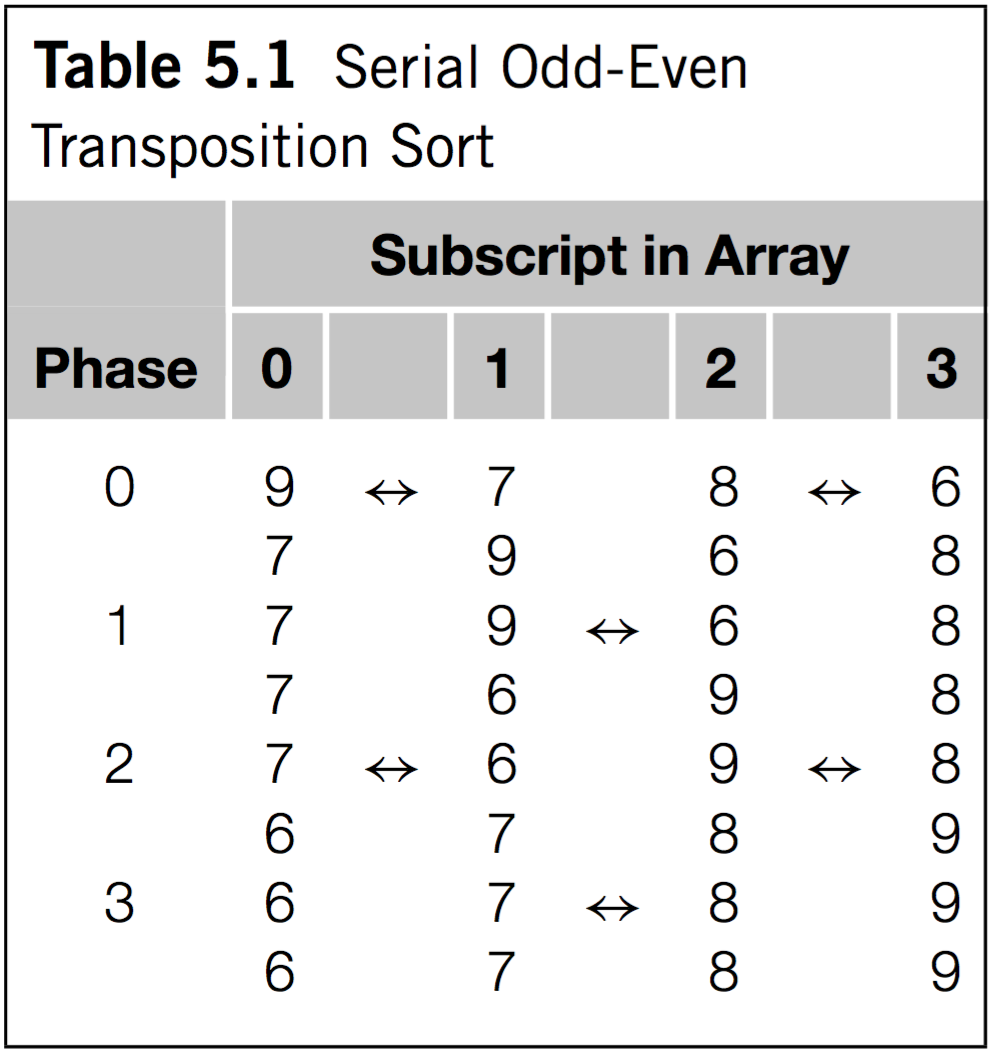
\includegraphics[width=0.35\textwidth]{img/pacheco/odd-even.png}
				\caption{Algoritmo de Ordenação Serial de Transposição Ímpar-Par.}
			\end{figure}
		\end{multicols}
\end{frame}

	\begin{frame}[fragile]{Odd-Even Transposition Sort - Loop-Carried Dependence}
		\begin{minted}[mathescape,linenos, numbersep=3pt, gobble=3, tabsize=3, frame=lines, framesep=2mm, fontsize=\footnotesize]{c}
			for (phase = 0; phase < n; phase++) 
				if (phase % 2 == 0)
					for (i = 1; i < n; i += 2)
						if (a[i 1] > a[i]) Swap(&a[i 1],&a[i]); 
				else
					for (i = 1; i < n 1; i += 2)
						if (a[i] > a[i+1]) Swap(&a[i], &a[i+1]);
		\end{minted}
		\begin{itemize}
			\item Exemplo
			\begin{itemize}
				\item Tem-se o vetor {\tt a =\{9, 7, 8, 6\}}. 
				\item Sequencial
				\begin{itemize}
					\item Na \textit{fase 0}: (9,7) e (8,6) resultando em \{7, 9, 6, 8\}.
					\item Na \textit{fase 1}: (6, 9) são permutados.
				\end{itemize}
				\item Paralelo executará todas as fases concorrentemente.
				\begin{itemize}
					\item na \textit{fase1}, será comparado o par (7,8) e não o (6, 9).
				\end{itemize}
			\end{itemize}
			\bigskip
			\item Já o loop interno não aparenta ter dependências.
		\end{itemize}
\end{frame}


			
	\begin{frame}{Odd-Even Transposition Sort - Impasses}
		\begin{itemize}
			\item Por mais que os loops internos não tenham nenhum tipo de dependência, deve-se antentar ao loop externo.
			\item Potencial 1:
			\begin{itemize}
				\item Deve-se ter certeza que todas as threads da \textit{fase p} terminaram antes do início de \textit{fase p+1}.
				\item Para que a diretiva {\tt parallel for} funcione, todos os threads de \textit{fase p} devem ter terminadas para a próxima iteração.
			\end{itemize}
			\item Potencial 2:
			\begin{itemize}
				\item \textit{Overhead} de \textit{forking} e \textit{joining} de threads.
			\end{itemize}
		\end{itemize}
	\end{frame}



	\begin{frame}[fragile]{Odd-Even Transposition Sort - Implementação 1}
		\begin{minted}[mathescape,linenos, numbersep=3pt, gobble=3, tabsize=3, frame=lines, framesep=2mm, fontsize=\scriptsize]{c}
			for (phase = 0; phase < n; phase++) { 
				if (phase % 2 == 0)
			#		pragma omp parallel for num_threads(thread_count) \ 
						default(none) shared(a, n) private(i, tmp)
					for(i=1;i<n;i+=2) { 
						if (a[i-1] > a[i]) {
							tmp = a[i-1]; 
							a[i-1] = a[i]; 
							a[i] = tmp;
						} 
					} else
			#		pragma omp parallel for num_threads(thread_count) \
						default(none) shared(a, n) private(i, tmp) 
					for(i=1;i<n 1;i+=2) {
						if (a[i] > a[i+1]) { 
							tmp = a[i+1]; 
							a[i+1] = a[i]; 
							a[i] = tmp;
						}
					}
			} 
		\end{minted}
\end{frame}


	\begin{frame}[fragile]{Odd-Even Transposition Sort - Implementação 2}
		\begin{minted}[mathescape,linenos, numbersep=3pt, gobble=3, tabsize=3, frame=lines, framesep=2mm, fontsize=\scriptsize]{c}
			# 	pragma omp parallel num_threads(thread_count) \ 
					default(none) shared(a, n) private(i, tmp, phase)
			for (phase = 0; phase < n; phase++) { 
				if (phase % 2 == 0)
			#		pragma omp for
					for(i=1;i<n;i+=2) { 
						if (a[i-1] > a[i]) {
							tmp = a[i-1]; 
							a[i-1] = a[i]; 
							a[i] = tmp;
						} 
					} else
			#		pragma omp for
					for(i=1;i<n 1;i+=2) {
						if (a[i] > a[i+1]) { 
							tmp = a[i+1]; 
							a[i+1] = a[i]; 
							a[i] = tmp;
						}
					}
			} 
		\end{minted}
\end{frame}


	\begin{frame}{Odd-Even Transposition Sort - Comparações}
		\begin{figure}[p]
			\centering
			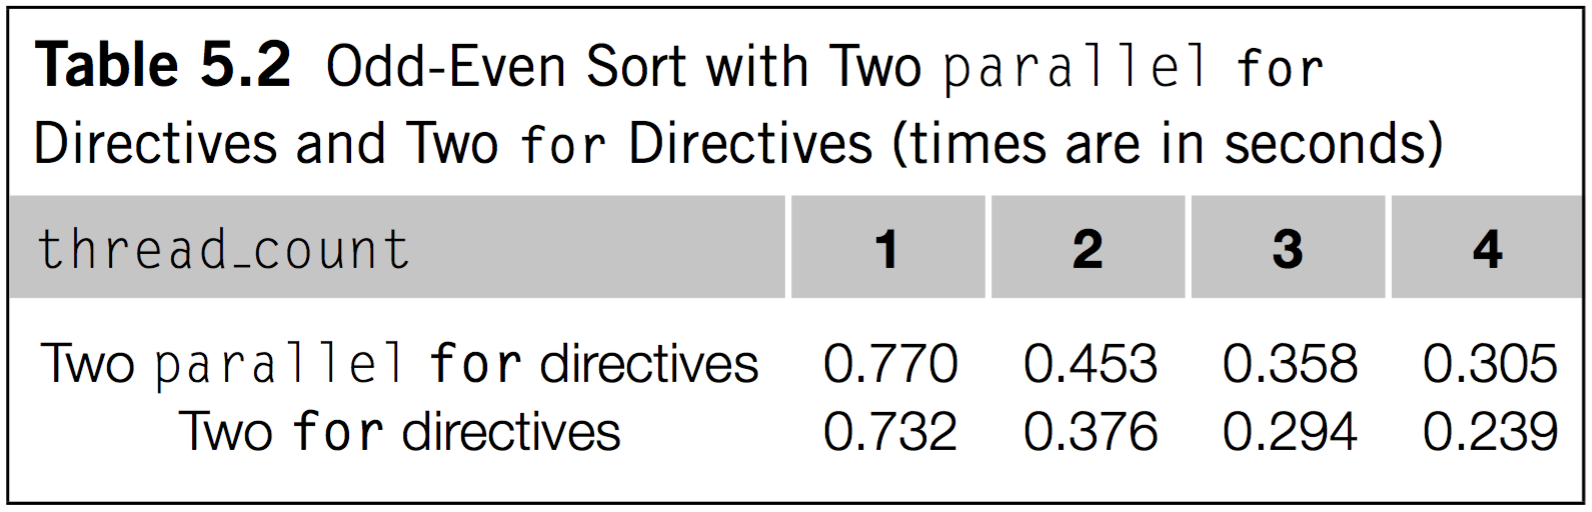
\includegraphics[width=0.5\textwidth]{img/pacheco/odd-even_comparation.png}
			\caption{Comparação entre o mesmo algoritmo sobre diretivas diferentes.}
		\end{figure}
		\begin{itemize}
			\item A diferença deve-se aos fatos
			\begin{itemize}
				\item O primeiro algoritmo realiza o \textit{forking} e \textit{joining} para cada iteração.
				\item Já o segundo reutiliza as mesmas threads já que q quantidade é sempre a mesma.
			\end{itemize}
			\item É possível criar um time de threads antes de loops com a diretiva {\tt parallel}.
			\item A diretiva {\tt for}, diferentemente de {\tt parallel for}, não \textit{fork} nehuma threads. Ela utiliza threads já prontas para uso.
			\item A segunda implementação obteve uma melhoria de $17\%$.
		\end{itemize}
	\end{frame}








	%5.7
\section{Escalonamento de Loops}
	\subsection{Escalonamento de Loops - Introdução}
	\begin{frame}[fragile]{Escalonamento de Loops - Introdução}
		\begin{itemize}
			\item A atribuição das iterações para as threads dependente do sistema.
			\item OpenMP possui uma implementação robusta de particionamento de bloco:
			\begin{itemize}
				\item $n$ iterações. Então $n/${\tt thread\_count} iterações serão atribuído a thread 0.
				\item Os próximos $n/${\tt thread\_count} serão atribuído a thread 1.
			\end{itemize}
			\item Existem inúmeras situações onde isso seria muito pouco ideal.
		\end{itemize}
		\begin{minted}[mathescape,linenos, numbersep=3pt, gobble=3, tabsize=3, frame=lines, framesep=2mm, fontsize=\small]{c}
			sum = 0.0;
			for (i = 0; i <= n; i++) 
				sum += f(i);
		\end{minted}
		\begin{itemize}
			%\todo{O que isso quer dizer 237}
			\item A divisão de blocos dará muito mais tarefas para a thread {\tt thread\_count} $-1$ do que a thread 0.
		\end{itemize}
\end{frame}

	\begin{frame}{Escalonamento de Loops - Introdução}
		\begin{itemize}
			\item Uma melhor atribuição é utilizando particionamento cíclico.
			\begin{itemize}
				\item A iteração é atribuída, uma em cada vez, no escalonamento ``round-robin''.
			\end{itemize}
		\end{itemize}

		\begin{multicols}{2}
			\begin{figure}[p]
				\centering
				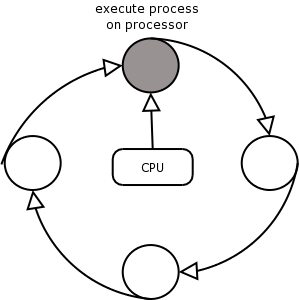
\includegraphics[width=0.3\textwidth]{img/pacheco/rr.png}
				\caption{Algoritmo de Escalonamento de Processo Round-Robin.}
			\end{figure}
		\columnbreak
			\begin{figure}[p]
				\centering
				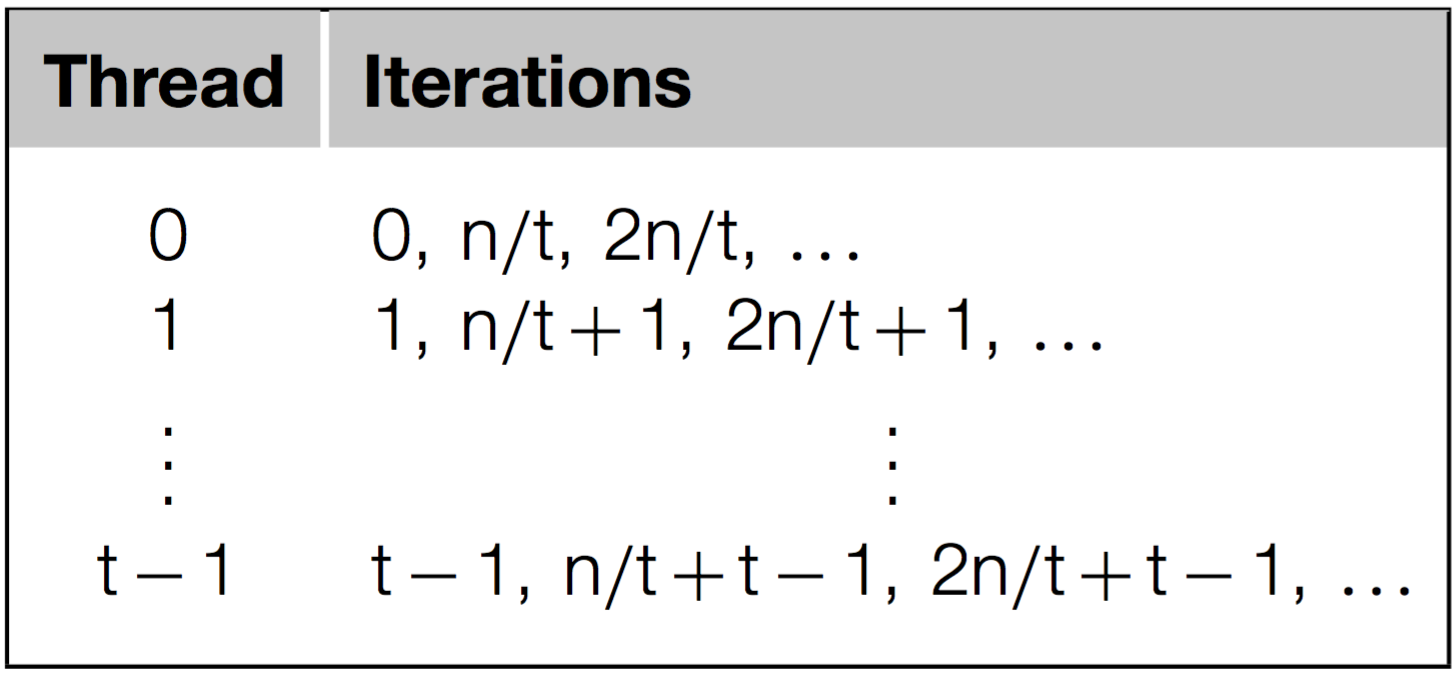
\includegraphics[width=0.5\textwidth]{img/pacheco/rr-threads.png}
				\caption{Divisão das iterações com o algoritmo Round-Robin.}
			\end{figure}
		\end{multicols}
	\end{frame}

	\begin{frame}[fragile]{Escalonamento de Loops - Comparação}
		\begin{itemize}
			\item Para ter noção de como isso afeta a performance, tem-se o seguinte programa
		\end{itemize}
		\begin{minted}[mathescape,linenos, numbersep=3pt, gobble=3, tabsize=3, frame=lines, framesep=2mm, fontsize=\scriptsize]{c}
			double f(int i) {
				int j, start = i*(i+1)/2, finish = start + i;
				double return_val = 0.0;
				for (j = start; j <= finish; j++) {
					return val += sin(j);
				}
				return return_val; 
			} /*f*/
		\end{minted}
		\begin{itemize}
			\item \textbf{Definição:} Se {\tt f(i)} leva tempo $i$, {\tt f(2i)} levará o dobro.
			\item \textbf{Sem escalonamento cíclico} com $n=10.000$:
			\begin{itemize}
				\item Uma única thread, leva-se $3,57s$.
				\item Duas threads, os blocos são divididos e leva-se $2,76s$. Speedup de 1,33.
			\end{itemize}
			\item \textbf{Com escalonamento cíclico} com $n=10.000$
			\begin{itemize}
				\item Com 2 threads vai para $1,84s$. Speedup de 1,99 e 1,5 respectivamente.
			\end{itemize}
			\item Existe a cláusula {\tt schedule} para diretivas {\tt for}.
		\end{itemize}
\end{frame}

	\subsection{Cláusula {\tt schedule}}
	\begin{frame}[fragile]{Cláusula {\tt schedule}}
		\begin{itemize}
			\item Escalonamento padrão usa-se a cláusula {\tt reduction} com algum {\tt for}.
		\end{itemize}
		\begin{minted}[mathescape,linenos, numbersep=3pt, gobble=3, tabsize=3, frame=lines, framesep=2mm, fontsize=\small]{c}
			sum = 0.0;
			# pragma omp parallel for num_threads(thread_count) \
				reduction(+:sum)		
			for (i = 0; i <= n; i++)
				sum += f(i);
		\end{minted}

		\begin{itemize}
			\item Para um escalonamento cíclico utiliza-se a cláusula {\tt schedule}
		\end{itemize}
		
		\begin{minted}[mathescape,linenos, numbersep=3pt, gobble=3, tabsize=3, frame=lines, framesep=2mm, fontsize=\small]{c}
			sum = 0.0;
			# pragma omp parallel for num_threads(thread_count) \
				reduction(+:sum) schedule(static.1)
			for (i = 0; i <= n; i++)
				sum += f(i);
		\end{minted}
\end{frame}

	\begin{frame}{Cláusula {\tt schedule}}
		\begin{itemize}
			\item Possui a forma {\tt schedule(<type> [, <chunksize>])} sendo:

			\item O parâmetro {\tt type}
			\begin{itemize}
				\item {\tt static}: Iterações podem ser atribuídas antes da sua execução;
				\item {\tt dynamic } ou {\tt guided}: Iterações podem ser atribuídas enquanto o loop é executado.
				\begin{itemize}
					\item Se depois que uma thread é completada na iteração atual, pode requisitar mais em tempo de execução.
				\end{itemize}
				\item {\tt auto}: O compilador e sistema determinará o escalonamento.
				\item {\tt runtime}: Será determinado em tempo de execução.
			\end{itemize}
			\item O parâmetro {\tt chunksize}
			\begin{itemize}
				\item Definição: \textit{chunk} de um iteração é um bloco de iterações que pode ser executado consecutivamente num loop serial.
				\item Definição: {\tt chunksize} é o número de iterações no bloco.
				\item Somente {\tt static}, {\tt dynamic} e {\tt guided} possuem essa opção.
			\end{itemize}
		\end{itemize}
	\end{frame}

	
	\begin{frame}{Cláusula {\tt schedule} - Static}
		\begin{itemize}
			\item O sistema atribui iterações \textit{chunk} de {\tt chunksize} para cada thread por meio do RR.
			\item Exemplo com 12 iterações ({\tt a = \{0, 1, ... , 11\})}
			\begin{itemize}
				\item \textbf{Se chunksize for 1} ({\tt schedule(static, 1)})
				\begin{itemize}
					\item \textbf{Thread 0:} 0, 3, 6, 9
					\item \textbf{Thread 1:} 1, 4, 7, 10
					\item \textbf{Thread 2:} 2, 5, 8, 11
				\end{itemize}
				\item \textbf{Se chunksize for 2} ({\tt schedule(static, 2)})
				\begin{itemize}
					\item \textbf{Thread 0:} 0, 1, 6, 7
					\item \textbf{Thread 1:} 2, 3, 8, 9
					\item \textbf{Thread 2:} 4, 5, 10, 11
				\end{itemize}
				\item \textbf{Se chunksize for 4} ({\tt schedule(static, 4)})
				\begin{itemize}
					\item \textbf{Thread 0:} 0, 1, 2, 3
					\item \textbf{Thread 1:} 4, 5, 6, 7
					\item \textbf{Thread 2:} 8, 9, 10, 11
				\end{itemize}
			\end{itemize}
			\item Se o {\tt chucksize} for omitido, será usado uma aproximação de $i/${\tt thread\_count}
		\end{itemize}
	\end{frame}

	
	\begin{frame}{Cláusula {\tt schedule} - Dynamic e Guided}
		\begin{itemize}
			\item Dynamic
			\begin{itemize}
				\item Iterações são quebradas em chunks de {\tt chunksize} de iterações consecutivas.
				\item Cada thread executa um chunk e quando ela termina, ela requisita outro em tempo de execução.
				\item Isso é executado até que as iterações sejam completadas.
			\end{itemize}
			\item Guided
			\begin{itemize}
				\item Tal como o Dynamic.
				\item Quando um chunk é completado, o tramanho do novo chunk é decrementado.
				\item Exemplo, no cálculo trapezoidal, se for calcular com intervalo de 10.000 e 2 threads: 
				\begin{itemize}
					\item A primeira thread ficará com $9999/2 \approx 5000$;
					\item A segunda ficará com $4999/2 \approx 2500$ e assim segue.
				\end{itemize}
			\end{itemize}
		\end{itemize}
	\end{frame}

	\begin{frame}{Cláusula {\tt schedule} - Dynamic e Guided}
		\begin{figure}[p]
			\centering
			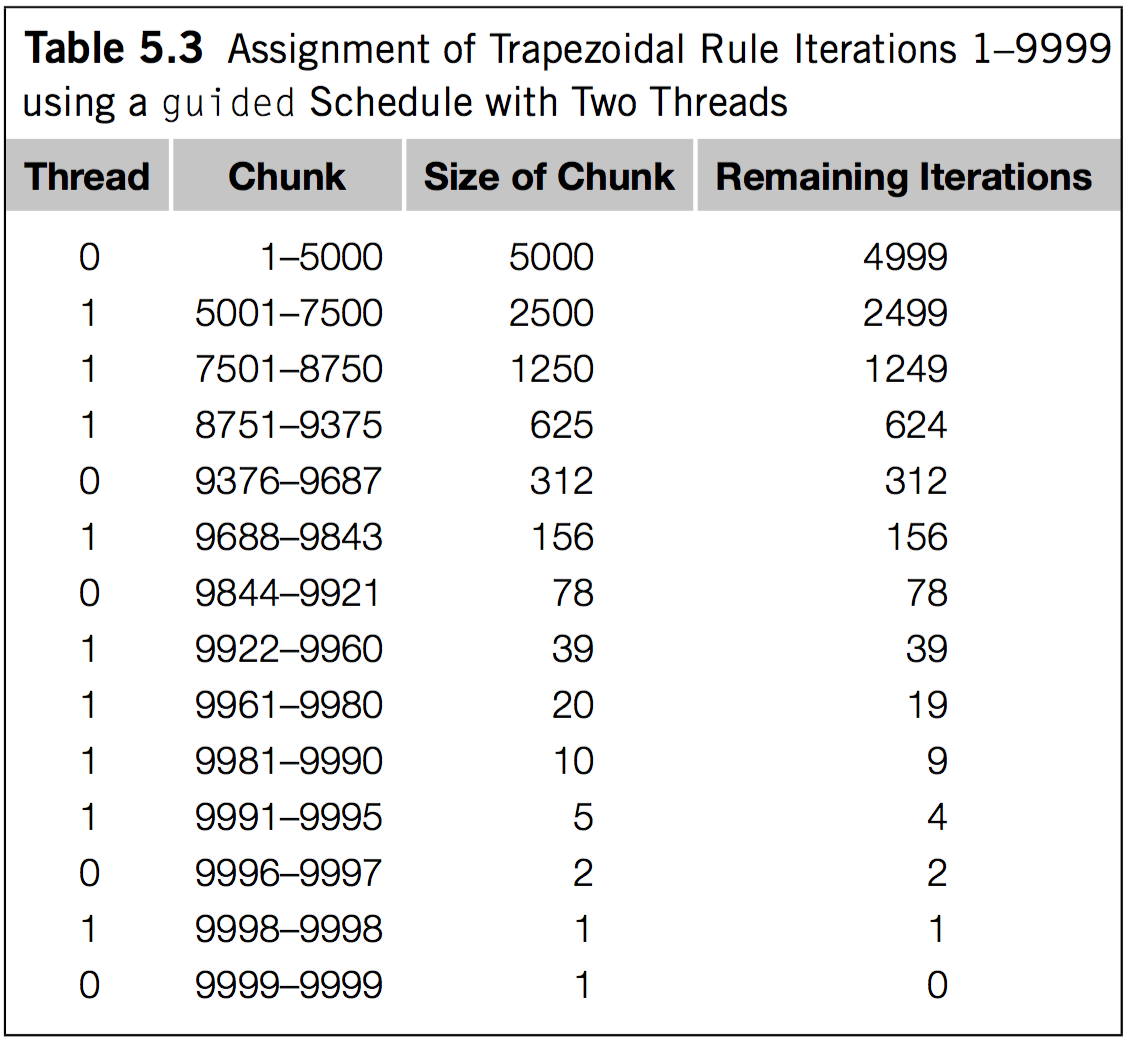
\includegraphics[width=0.52\textwidth]{img/pacheco/dynamic-guided.png}
			\caption{Tabela de da quantidade de chunks.}
		\end{figure}
	\end{frame}

	\begin{frame}{Cláusula {\tt schedule} - runtime}
		\begin{itemize}
			\item Antes, deve-se definir variável de ambientem: Valores nomeados que podem ser acessados em tempo de execução. Disponívels no ambiente do programa.
			\item Quando {\tt schedule(runtime)} é especificado, o sistema utiliza a variável de ambiente {\tt OMP\_SCHEDULE}.
			\begin{itemize}
				\item Ela pode ter qualquer valor que poderia ser usado em {\tt static, dynamic}, ou {\tt guided}.
				\item {\tt \$ export OMP\_SCHEDULE=``static,1''}
			\end{itemize}
		\end{itemize}
	\end{frame}

	\begin{frame}{Cláusula {\tt schedule} - Como decidir?}
		\begin{itemize}
			\item Que tipo de escaolonamento e chunksize deveriamos usar?
					\bigskip
			\item Como é possível perceber, existe alguns tipos de overheads em alguns tipos de escalonamento.
			\item A sobrecarga é maior para dynamic do que static.
			\item Há sobrecarga no guided em árvores.
					\bigskip
			\item Se deseja-se um desempenho satisfatório sem o uso de {\tt schedule}, deve-se ir além.
			%\todo{Abordagens diferentes}
			\item Caso contário, se achar que o escalonamento pode ser melhorado, deverá tentar abordagens diferentes.
			\item Como no primeiro exemplo, se a melhoria de 1,99 de speed up é satisfatório, deve-se parar.
			\item Entretanto, se for variar o número de threads e o número de iterações, deve ser experimentado outras possibilidades.
			\item Achar o `ótimo escalonável' está diretamente relacionado ao número dde iterações e threads.
					\bigskip
			\item Se a performance do escalonador padrão não tiver aceitável, pode-se trocar o tipo de escaolonador
			\begin{itemize}
				\item Existe uma lista ampla de escalonadores.
			\end{itemize}
			\item Mesmmo assim, pode ter a possibilidade do loop não ser muito bem paralelizável ou nenhum escalonador dará a performace requerida.
		\end{itemize}
	\end{frame}

	\begin{frame}{Cláusula {\tt schedule} - Explorar Escalonadores}
		\begin{itemize}
			\item Algumas ideias para explorar alguns escalonadores antes de outros
			\begin{enumerate}
				\item Se cada iteração exige a mesma quantidade de computação, então o padrão dará melhor performance.
				\item Se o custo das iterações cresce ou decresce de forma linear, então o {\tt static} com chunksize pequeno dará grande performance.
				\item Se o custo não pode ser determinado, então pode-se fazer variações de escalonamento. O {\tt schedule(runtime)} também pode ser utilizado também.
			\end{enumerate}
		\end{itemize}
	\end{frame}









\section{Produtor e Consumidor}
	\begin{frame}{Introdução}
		\begin{itemize}
			\item Um olhar sobre paralelismo em atividades que não são fáceis de lidar usando a diretiva {\tt parallel for} ou {\tt for}.
			\bigskip
			\item Fila é uma estrutura de dados natural usado em várias aplicações multithreads.
			\begin{itemize}
				\item Um exemplo é o produtor e consumidor.
				\item Neste exemplo, o processo não pode ser terminado sem que todos os recursos não foram consumidos.
			\end{itemize}
			\item Troca de mensagem por memória compartilhada:
			\begin{itemize}
				\item Cada thread deve ter uma fila de memória compartilhada.
				\item Quando uma thread quer enviar uma mensagem para outra thread, `enfilera' a mensagem na fila do destinatário.
			\end{itemize}
			\item Supondo um implementação simples de troca de mensagem no qual
			\begin{itemize}
				\item Cada thread irá gerar um número inteiro randômico que serão as mensagens;
				\item E um número randômico de destinatários.
				\item Passos:
				\begin{enumerate}
					\item Depois de criado as mensagens, cada thread checará sua própria lista de mensagens;
					\item Se tiver mensangem, retira da fila e imprime na na tela;
					\item Cada thread alternará entre tentar enviar e receber mensagens;
					\item O usuário definirá o número de mensagens que cada thread deve enviar;
					\item Quando uma thread enviar todas as mensangens, ela ficará recebendo mensagens até que todas acabarem também e serão fechadas.
				\end{enumerate}
			\end{itemize}
		\end{itemize}
	\end{frame}

	\begin{frame}[fragile]{Troca de Mensagem -  Pseudocódigo}
		\begin{minted}[mathescape,linenos, numbersep=3pt, gobble=3, tabsize=3, frame=lines, framesep=2mm, fontsize=\normalsize]{c}
			for (sent_msgs = 0; sent_msgs < send_max; sent_msgs++) { 
				Send_msg();
				Try_receive();
			}
			
			while (!Done()) 
				Try receive();
		\end{minted}
\end{frame}

	\begin{frame}[fragile]{Troca de Mensagem -  Envio de mensagens}
		\begin{itemize}
			\item Acessar uma fila de mensagem provavelmente é uma seção crítica.
			\item Por mais que não olhemos os detalhes da implementação da fila, deve-se tomar medidas de prevenção usando seção crítica.
			\item Pseudocódigo do {\tt Send\_msg()}
		\end{itemize}
		\begin{minted}[mathescape,linenos, numbersep=3pt, gobble=3, tabsize=3, frame=lines, framesep=2mm, fontsize=\normalsize]{c}
			mesg = random();
			dest = random() % thread_count;
			#	pragma omp critical
			Enqueue(queue, dest, my_rank, mesg);
		\end{minted}
		\begin{itemize}
			\item É permitido que a thread envie mensagem pra si mesmo.
		\end{itemize}
\end{frame}
	\begin{frame}[fragile]{Troca de Mensagem -  Recebimento de mensagens}
		\begin{itemize}
			\item A questão de sincronização para recebimento de mensagens é diferente do envio.
			\item Dono de sua própria fila, irá retirar uma a uma.
			\item Se existe pelo menos duas mensagens na fila, a {\tt Dequeue} não pode conflitar com {\tt Enqueue}.
			\begin{itemize}
				\item Mantendo o controle da fila, mantém-se a sincronização.
			\end{itemize}
					\bigskip
			\item Mas, e a variável que armazena o tamanho da lista?
			\item Tem-se 2 variáveis com o número de mensagens
		\end{itemize}
		\begin{minted}[mathescape,linenos, numbersep=3pt, gobble=3, tabsize=3, frame=lines, framesep=2mm, fontsize=\normalsize]{c}
			queue_size = enqueued - dequeued
		\end{minted}
		\begin{itemize}
			\item {\tt dequeued} é atualizado por seu próprio dono.
			\item Entrentanto, uma thread pode estar atualizando {\tt enqueued} enquando outra usa o valor de {\tt queue\_size}
		\end{itemize}
\end{frame}

	\begin{frame}[fragile]{Troca de Mensagem -  Recebimento de mensagens}
		\begin{itemize}
			\item Assim, o {\tt Try\_receive} será implementado
		\end{itemize}
		\begin{minted}[mathescape,linenos, numbersep=3pt, gobble=3, tabsize=3, frame=lines, framesep=2mm, fontsize=\normalsize]{c}
			queue_size = enqueued - dequeued;

			if (queue_size == 0) 
				return;

			else if (queue_size == 1)
				#	pragma omp critical
				Dequeue(queue, &src, &mesg);

			else
				Dequeue(queue, &src, &mesg);

			Print_message(src, mesg);
		\end{minted}
\end{frame}

	\begin{frame}[fragile]{Troca de Mensagem -  Detecção de Término}
		\begin{itemize}
			\item Deve-se verificar o fim da execução do processo.
		\end{itemize}


		\begin{multicols}{2}
			\begin{itemize}
				\item É fácil percebe que esta implementação possui problemas.
				\begin{itemize}
					\item Quando uma thread \textit{u} estiver computado que {\tt queue\_size == 0}, outra thread \textit{v} provavelmente enviará uma mensagem.
					\item Se isso acontecer, a mensagem enviada nunca será lida.
				\end{itemize}
				\item Para isso, utiliza um {\tt done\_sending} que será incrementado a cada finaliação de envio das threads. Permitindo a implementação
			\end{itemize}
		\columnbreak
			\begin{minted}[mathescape,linenos, numbersep=3pt, gobble=4, tabsize=3, frame=lines, framesep=2mm, fontsize=\footnotesize]{c}
				queue_size = enqueued - dequeued; 

				if (queue_size == 0)
					return TRUE; 
				else return FALSE;
			\end{minted}
					\pause
			\begin{minted}[mathescape,linenos, numbersep=3pt, gobble=4, tabsize=3, frame=lines, framesep=2mm, fontsize=\footnotesize]{c}
				queue_size = enqueued - dequeued; 

				if (queue_size == 0 && 
								done_sending == thread_count)
					return TRUE; 
				else return FALSE;
			\end{minted}
		\end{multicols}
\end{frame}


	\begin{frame}{Troca de Mensagem -  Iniciando}
		\begin{itemize}
			\item Quando o programa inicia, é recebido por parâmetro a quantidade de threads.
			\item Também é alocado a fila de mensagens, uma para cada thread.
			\begin{itemize}
				\item Este arranjo precisa ser compartilhado entre as threads.
			\end{itemize}
			\item Existirá os seguintes armazenamentos;
			\begin{itemize}
				\item Lista de mensagem;
				\item Um ponteiro para o índice da cauda da fila;
				\item Um ponteiro para o índice da cabeça da fila;
				\item Um contaor de mensagens enfileiradas; e
				\item Um contador de mensagens desenfileiradas.
			\end{itemize}
			\item Após a alocação, pode-se iniciar as threadas usando a diretiva {\tt parallel} e cada uma alocando sua fila individual.
		\end{itemize}
	\end{frame}

	\begin{frame}{Troca de Mensagem -  Iniciando}
		\begin{itemize}
			\item É provável que aconteça que algumas threads acabará de alocar antes das outras e começará a enviar as mensagens mesmo que outras threads não tenham terminado a alocação.
			\begin{itemize}
				\item \textit{Segmentation Fault}.
			\end{itemize}
			\item Deve-se fazer com que nenhuma thread começe antes que todas tenham alocado. E com isso utiliza-se barreiras.
			\begin{itemize}
				\item Enquanto todas as threads do time não completarem a ação, as outras não podem continuar.
				\item Esta barreira é explícita sendo sua diretiva
			\end{itemize}
			{\tt \#	pragma omp barrier}
		\end{itemize}
	\end{frame}

	\begin{frame}{Troca de Mensagem -  Diretiva atomic}
		\begin{itemize}
			\item Após completado as diretivas de envio, cada thread incrementa {\tt done\_sending} no final do loop.
			\item {\tt done\_sending} é uma seção crítica e poderíamos protegê-la com a diretiva {\tt critical}.
			\item Mas OpenMP provê uma diretiva potencialmente de alta performance. A diretiva atômica.
		\end{itemize}
		{\tt \#	pragma omp atomic}
	\end{frame}

	\begin{frame}[fragile]{Troca de Mensagem -  Diretiva atomic}
		\begin{itemize}
			\item Ao contrário da {\tt critical}, ela só protege seções críticas que consistem numa única atribuição. Tal como:
			\begin{verbatim}
				x <op>= <expression>;
				x++;
				++x;
				x--;
				--x;\end{verbatim}
			\item Sendo {\tt <op>} um operador binário: \verb%+, *, -, /, &, ^, |, <<,% ou \verb%>>% e {\tt <expression>} não pode referenciar {\tt x}.
			\item A expressão não está inclusa na seção crítica. Somente a atribuição do resultado dela à variável que está.
		\end{itemize}

		\begin{minted}[mathescape,linenos, numbersep=3pt, gobble=3, tabsize=3, frame=lines, framesep=2mm, fontsize=\footnotesize]{c}
			#	pragma omp atomic
				x += y++;
		\end{minted}
\end{frame}

	\begin{frame}{Troca de Mensagem -  Seção Crítica e locks}
		\begin{itemize}
			\item Algumas precauções sobre a diretiva {\tt critical}.
			\item Em todo os exemplos, existe mais de uma seção crítica.
			\item Entretanto, o uso de seção crítica na passagem de mensagens é mais complexa.
			\item Se examinarmos existe 3 blocos que utilizam diretivas {\tt critical} e {\tt atomic}
			\begin{itemize}
				\item {\tt done\_sending++;}, {\tt Enqueue(q\_p, my\_rank, mesg);} e {\tt Dequeue(q\_p, \&src, \&mesg);}.
			\end{itemize}
			\item Entretanto, não é necessário que as três tenha completo acesso exclusivo. Inclusive as duas últimas.
			\begin{itemize}
				\item Seria viável a threado 0 enfileirar uma mensagem na thread 1 enquanto esta enfilera uma mensagem em thread 2.
			\end{itemize}
			\item OpenMP provês duas seções críticas distintas. O {\tt atomic} e o `composto' de seções críticas que enfileiramos e retiramos mensagens.
			\item Desde que aplique exclusão mútua entre as threads de execução seriável, esse é o comportamento principal do OpenMP.
			\begin{itemize}
				\item Todas os blocos de seções críticas são parte de um composto de seção crítica.
			\end{itemize}
		\end{itemize}
	\end{frame}

	\begin{frame}[fragile]{Troca de Mensagem -  Seção Crítica e locks}
		\begin{itemize}
			\item É possível dar um nome a diretiva crítica: \verb%#	pragma omp critical(name)%.
			\item Fazendo isso, dois blocos protegidos com {\tt critical} com diferentes nomes podem executar simultaneamente.
			\begin{itemize}
				\item Os nomes são definitos em tempo de compilação;
			\end{itemize}
			\item Entretanto, perecisamos definir algo que seja em tempo de execução. E por esse motivo, nomear {\tt critical} não é suficente.
			\item Uma alternativa é utilizar locks.
		\end{itemize}
\end{frame}

	\begin{frame}[fragile]{Troca de Mensagem -  Lock}
		\begin{itemize}
			\item Lock consistem de estruturas de dados e funções que permitem o programador explicitar a exclusão mútua numa seção crítica.
			\item O uso do lock pode ser descrito pelo seguinte pseudocódigo:
		\end{itemize}
		\begin{minted}[mathescape,linenos, numbersep=3pt, gobble=3, tabsize=3, frame=lines, framesep=2mm, fontsize=\scriptsize]{c}
			/* Executed by one thread */
			Initialize the lock data structure;
			...
			/* Executed by multiple threads */
			Attempt to lock or set the lock data structure; Critical section;
			Unlock or unset the lock data structure;
			...
			/* Executed by one thread */
			Destroy the lock data structure;
		\end{minted}
		\begin{itemize}
			\item Inicialização
			\begin{itemize}
				\item A estrutura de dados é compartilhada com as threads que irão executar a seção crítica.
				\item A thread master irá inicializar o lock. Quanto todas estiver utilizando, uma deverá qubrá-lo.
			\end{itemize}
			\item Execução
			\begin{itemize}
				\item Depois que uma entrar na seção crítica, começa a tentativa de \textit{definir} a estrutura de dados lock chamando a função lock.
				\item Se nenhuma outra thread estiver executando o código da seção crítica, ela obtém o lock e procede para a seção crítica passando a chamada para a função lock.
				\item Quando a thread finaliza, ela chama a função unlock. Isso permitirá que outra thread possa obter o lock.
			\end{itemize}
		\end{itemize}
\end{frame}

	\begin{frame}{Cláusula {\tt schedule} - Lock}
		\begin{figure}[p]
			\centering
			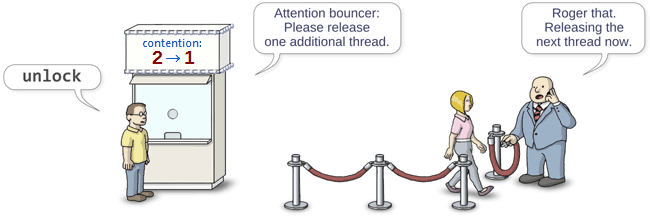
\includegraphics[width=1\textwidth]{img/pacheco/mutex.png}
			\caption{Exemplo de lock.}
		\end{figure}
	\end{frame}

	\begin{frame}{Cláusula {\tt schedule} - Lock}
		\begin{figure}[p]
			\centering
			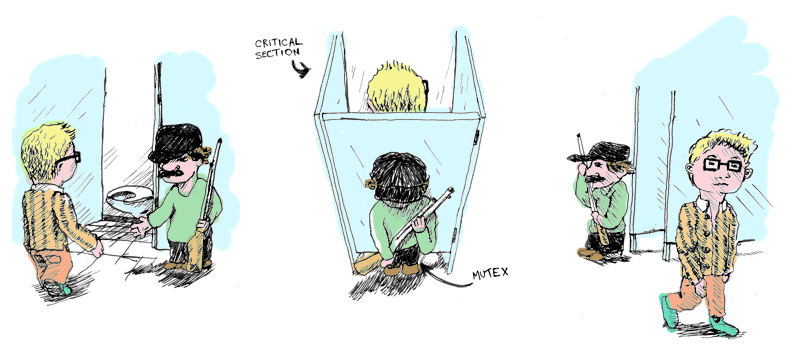
\includegraphics[width=1\textwidth]{img/pacheco/mutex2.png}
			\caption{Outro exemplo de lock.}
		\end{figure}
	\end{frame}

	\begin{frame}[fragile]{Troca de Mensagem -  Lock}
		\begin{itemize}
			\item OpenMP possui dois tipos de lock
			\begin{itemize}
				\item Simple: Pode ser `setado' somente depois que for `des-setado'.
				\item Nested: Pode ser definido múltilas vezes pela mesma thread antes do `des-set'.
			\end{itemize}
			\item Um tipo de OpenMP simple lock é o {\tt omp\_lock\_t}, e e possui as funções de definição:
			\begin{minted}[mathescape,linenos, numbersep=3pt, gobble=4, tabsize=3, frame=lines, framesep=2mm, fontsize=\small]{c}
				void omp_init_lock(omp_lock_t *    lock_p /* out */);
				void omp_set_lock(omp_lock_t *     lock_p /* in/out */); 
				void omp_unset_lock(omp_lock_t *   lock_p /* in/out */);  
				void omp_destroy_lock(omp_lock_t * lock_p /* in/out */);    
			\end{minted}
			\item Tudo isso é especificado em {\tt omp.h}.
		\end{itemize}
\end{frame}


	\begin{frame}[fragile]{Troca de Mensagem -  Lock}
		\begin{itemize}
			\item Queremos assegurar a exclusão mútua em cada fila de mensagem e não em um bloco de código particular.
			\item Pode-se trocar os códigos
		\end{itemize}

		\begin{multicols}{2}
				\begin{minted}[mathescape,linenos, numbersep=3pt, gobble=5, tabsize=3, frame=lines, framesep=2mm, fontsize=\small]{c}
					#	pragma omp critical
						/*q_p = msg_queues[dest]*/
						Enqueue(q_p, my_rank, mesg);
				\end{minted}
			\begin{itemize}
				\item Por
			\end{itemize}
				\begin{minted}[mathescape,linenos, numbersep=3pt, gobble=5, tabsize=3, frame=lines, framesep=2mm, fontsize=\small]{c}
						/*q_p = msg_queues[dest]*/
						omp_set_lock(&q_p->lock);
						Enqueue(q_p, my_rank, mesg);
						omp_unset_lock(&q_p->lock);
				\end{minted}
		\columnbreak
				\begin{minted}[mathescape,linenos, numbersep=3pt, gobble=5, tabsize=3, frame=lines, framesep=2mm, fontsize=\footnotesize]{c}
					#	pragma omp critical
						/*q_p = msg_queues[my_rank]*/
						Dequeue(q_p, &src, &mesg);
				\end{minted}
			\begin{itemize}
				\item Por
			\end{itemize}
				\begin{minted}[mathescape,linenos, numbersep=3pt, gobble=5, tabsize=3, frame=lines, framesep=2mm, fontsize=\small]{c}
						/*q_p = msg_queues[my_rank]*/
						omp_set_lock(&q_p->lock);
						Dequeue(q_p, &src, &mesg);
						omp_unset_lock(&q_p->lock);
				\end{minted}
		\end{multicols}
\end{frame}

	\begin{frame}{Diretiva {\tt critical}, Diretiva {\tt atomic} ou lock}
		\begin{itemize}
			\item A diretiva {\tt atomic} é potencialmente mais rápida para obter exclusão mútua.
			\item Se a seção crítica consiste numa atribuição que querer uma forma, então utiliza-se tão bem o atomic quanto as outras.
			\item Impões exclusão mútua a todas as diretivas {\tt atomic}. Essa é a forma que a {\tt critical} sem nomeação comporta.
			\item Se isso pode ser um problema, por exemplo, ter várias seções críticas diferentes, então deve-se utilizar {\tt critical} nomeado ou locks.
		\end{itemize}
	\end{frame}


	\begin{frame}[fragile]{Diretiva {\tt critical}, Diretiva {\tt atomic} ou lock}
		\begin{itemize}
			\item Supondo que cada um dos códigos abaixo é executado em duas threads diferenes
		\end{itemize}

		\begin{multicols}{2}
				\begin{minted}[mathescape,linenos, numbersep=3pt, gobble=5, tabsize=3, frame=lines, framesep=2mm, fontsize=\small]{c}
					#	pragma omp critical
						x++;
				\end{minted}
		\columnbreak
				\begin{minted}[mathescape,linenos, numbersep=3pt, gobble=5, tabsize=3, frame=lines, framesep=2mm, fontsize=\footnotesize]{c}
					#	pragma omp critical
						y++;
				\end{minted}
		\end{multicols}
		\begin{itemize}
			\item Mesmo se tiverem em locais de memória diferente, se uma thread executa o código a esquerda então nenhum outro executa a direita.
			\item Entretanto, ambas as {\tt critical} (nomeadas e não nomeadas) são fácels de trabalhar.
			\item Não existe uma diferença significativa entre a {\tt critical} e locks.
			\begin{itemize}
				\item Se não pode utilizar uma diretiva atômica, qualquer uma das duas satisfaz.
			\end{itemize}
			\item Locks deve ser usado quando é necessária a exclusão mútua para uma \textbf{estrutura de dados} em vez de um \textbf{bloco de código}.
		\end{itemize}
\end{frame}

	\begin{frame}[fragile]{Ressalvas}
		\begin{itemize}
			\item Não deve juntar diferentes tipos de de exlusão para uma única seção.
			\begin{multicols}{2}
				\begin{minted}[mathescape,linenos, numbersep=3pt, gobble=5, tabsize=3, frame=lines, framesep=2mm, fontsize=\normalsize]{c}
					#	pragma omp atomic
						x += f(y);
				\end{minted}
			\columnbreak
				\begin{minted}[mathescape,linenos, numbersep=3pt, gobble=5, tabsize=3, frame=lines, framesep=2mm, fontsize=\normalsize]{c}
					#	pragma omp critical
						x = g(x);
				\end{minted}
			\end{multicols}
			\begin{itemize}
				\item A atualização de {\tt x} à direita não tem uma forma definida pela diretiva {\tt atomic} e por isso utilizou o {\tt critical}.
				\item O {\tt critical} não excluirá a ação do {\tt atomic} gerando possível resultados incorretos.
				\item Deve-se reescrever a função {\tt g()} pra que seja da forma da diretiva {\tt atomic}, ou proteger ambos os blocos com {\tt critical}.
			\end{itemize}
		\end{itemize}
\end{frame}

	\begin{frame}[fragile]{Ressalvas}
		\begin{itemize}
			\item Não existe garantia de justiça na construção de exclusão mútua.
			\begin{minted}[mathescape,linenos, numbersep=3pt, gobble=4, tabsize=3, frame=lines, framesep=2mm, fontsize=\normalsize]{c}
					while (1) {
						...
				#		pragma omp critical
						x = g(my_rank);
						...
					}
			\end{minted}
			\begin{itemize}
				\item Uma thread pode ser bloqueada pra sempre esperando a seção crítica.
			\end{itemize}
		\end{itemize}
\end{frame}

	\begin{frame}[fragile]{Ressalvas}
		\begin{itemize}
			\item Pode ser perigoso aninhar exclusões mútuas
			\begin{itemize}
				\item Isso é uma garantia para \textbf{deadlock}.
				\item Quando uma thread tenta entrar na segunda seção crítica, ela fica bloqueada pra sempre.
				\item Se uma thread $u$ está executando dentro da primeira seção crítica, nenhuma thread pode estar dentro da segunda.
				\item A thread $u$ espera a segunda seção crítica e a thread $v$, dentro da segunda,  espera a primeira.
			\end{itemize}

			\begin{multicols}{2}
				\begin{minted}[mathescape,linenos, numbersep=3pt, gobble=5, tabsize=3, frame=lines, framesep=2mm, fontsize=\small]{c}
					#	pragma omp critical
						y = f(x);
						...
						double f(double x) {
					#		pragma omp critical
							z = g(x); // z is shared
						}
				\end{minted}
			\columnbreak
				\pause
				\begin{minted}[mathescape,linenos, numbersep=3pt, gobble=5, tabsize=3, frame=lines, framesep=2mm, fontsize=\small]{c}
					#	pragma omp critical(one)
						y = f(x);
						...
						double f(double x) {
					#		pragma omp critical(two)
							z = g(x); // z é global
						}
				\end{minted}
			\end{multicols}
		\end{itemize}
\end{frame}

	\begin{frame}[fragile]{Ressalvas}
		\begin{multicols}{2}
			\begin{minted}[mathescape,linenos, numbersep=3pt, gobble=4, tabsize=3, frame=lines, framesep=2mm, fontsize=\footnotesize]{c}
				#	pragma omp critical
					y = f(x);
					...
					double f(double x) {
				#		pragma omp critical
						z = g(x); // z is shared
					}
			\end{minted}
		\columnbreak
			\begin{minted}[mathescape,linenos, numbersep=3pt, gobble=4, tabsize=3, frame=lines, framesep=2mm, fontsize=\footnotesize]{c}
				#	pragma omp critical(one)
					y = f(x);
					...
					double f(double x) {
				#		pragma omp critical(two)
						z = g(x); // z é global
					}
			\end{minted}
		\end{multicols}

		\begin{figure}[p]
			\centering
			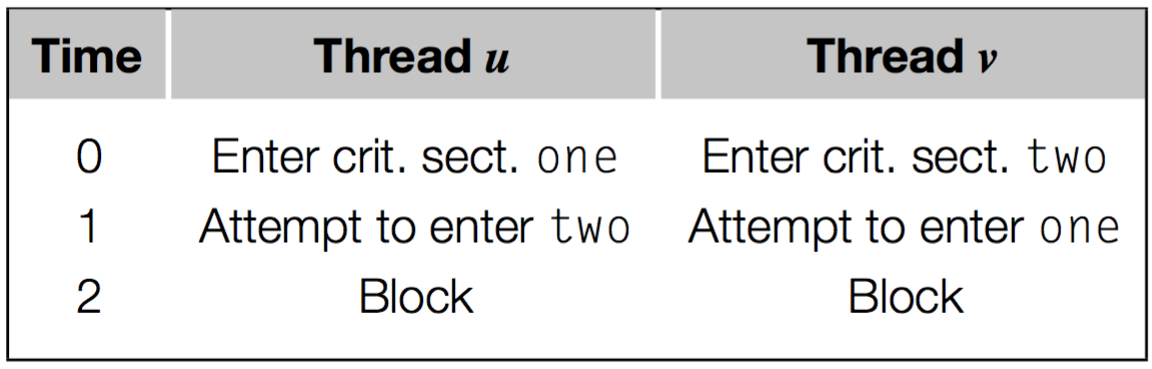
\includegraphics[width=0.6\textwidth]{img/pacheco/deadlock.png}
			\caption{Deadlock.}
		\end{figure}
\end{frame}











\section{Thread-Safefy}
	\subsection{Introdução}
	\begin{frame}[fragile]{Introdução}
		\begin{itemize}
			\item Outro problema que ocorre com o compartilhamento de memória é o thead-safety.
			\item Um bloco de código é thread-safety se pode ser executado simultaneamente por várias threads sem causar problemas.
			\item Um exemplo é múltiplas threads ``tokenizear'' um arquivo.
			\item Uma abordagem seria dividir o arquivo em linhas de texto e colocar cada thread para executar com escalonamento round-robin.
			\item Existindo $n$ linhas
			\begin{itemize}
				\item Thread 0 fica com $n$;
				\item Thread 1 fica com $n+1$;
				\item Thread t fica com $n+t$;
				\item Thread 0 fica com $n+t+1$ e segue;
			\end{itemize}
		\end{itemize}
\end{frame}

	\begin{frame}[fragile]{Introdução}
		\begin{itemize}
			\item Existe a função {\tt strtok} no {\tt string.h}.
			\item Ela retorna tokens de acordo com separador definido. Segue o seguinte protótipo
		\end{itemize}
		\begin{minted}[mathescape,linenos, numbersep=3pt, gobble=3, tabsize=3, frame=lines, framesep=2mm, fontsize=\footnotesize]{c}
			char * strtok(char* string /* in/out */, 
						  const char * separators /* in */);
		\end{minted}
		\begin{itemize}
			\item Seu uso é um pouco incomum
			\begin{itemize}
				\item Devemos passar a cadeia \verb%\t\n% como o argumento separadores dos tokens.
				\item A primeira vez que ele é chamado, o argumento {\tt string} deve ser o texto a ser indexado.
				\item Para chamadas subsequêntes, {\tt string} deverá ser NULL. 
				\item Assim, na primeira chamada, {\tt strtok()} armazena o ponteiro e para chamadas seguintes ele retorna tokens de sucessivas tomadas a partir da cópia em cache.
			\end{itemize}
		\end{itemize}
\end{frame}

	\begin{frame}[fragile]
		\begin{minted}[mathescape,linenos, numbersep=3pt, gobble=3, tabsize=3, frame=lines, framesep=2mm, fontsize=\footnotesize]{c}
			void Tokenize(
					char* lines[] /* in/out */, int line count /* in */, int thread_count /* in */) {
				int my_rank, i, j; char *my_token;
			#	pragma omp parallel num_threads(thread_count) \ 
						default(none) private(my_rank, i, j, my_token) \ 
						shared(lines, line_count)
				{
					my_rank = omp_get_thread_num(); 
			#		pragma omp for schedule(static, 1) 
					for (i = 0; i < line_count; i++) {
						printf("Thread %d > line %d = %s", my_rank, i, lines[i]);
						j = 0;
						my_token = strtok(lines[i], "\t\n");
						while ( my_token != NULL ) {
							printf("Thread %d > token %d = %s\n", my_rank, j, my_token);
							my_token = strtok(NULL, " \t\n");
							j++;
						}
					} /* for i */
				} /* omp parallel */
			} /* Tokenize */
		\end{minted}
\end{frame}

	\begin{frame}[fragile]{Introdução}
		\begin{itemize}
			\item Executando a primeira vez o código com duas threads e com 4 entradas: ``Pease porridge hot.'' ``Pease porridge cold.'' ``Pease porridge in the pot'' ``Nine days old.''.
			\begin{itemize}
				\item Obtêm o resultado corretamente.
			\end{itemize}

			\item Ao executar pela segunda vez obtêm o seguinte resultado
			\begin{verbatim}
Thread 0 > line 0 = Pease porridge hot.
Thread 1 > line 1 = Pease porridge cold.
Thread 0 > token 0 = Pease
Thread 1 > token 0 = Pease
Thread 0 > token 1 = porridge
Thread 1 > token 1 = cold.
Thread 0 > line 2 = Pease porridge in the pot 
Thread 1 > line 3 = Nine days old.
Thread 0 > token 0 = Pease 
Thread 1 > token 0 = Nine 
Thread 0 > token 1 = days 
Thread 1 > token 1 = old.
			\end{verbatim}
		\end{itemize}
\end{frame}

	\begin{frame}
		\begin{itemize}
			\item O que aconteceu?
			\begin{itemize}
				\item Apesar {\tt lines} ser argumento só de entrada, {\tt strtok} modifica o vetor.
				\item Quando {\tt Tokenize} retornar o vetor {\tt lines} estará modificado pois {\tt strtok} armazena em cache a linha de entrada. 
				\item {\tt strtok} armazena os valores numa variável estática persistindo-a. 
				\item Essa persistência é `cache compartilhado'.
				\item A thraead 0 encontrou um token ({\tt dias}) que deveria estar na saída da thraead 1.
			\end{itemize}
			\item Portanto, {\tt strtok} não é thread-safety.
			\item Isso não é incomum nas funções das bibliotecas em C.
			\begin{itemize}
				\item Gerador de número randômico do {\tt stdlib.c} e a função de conversão de tempo local {time.c} também falham.
			\end{itemize}
		\end{itemize}
	\end{frame}

	\begin{frame}[fragile]
		\begin{itemize}
			\item Em alguns casos o  padrão C especifica suplentes.	
		\end{itemize}

		\begin{minted}[mathescape,linenos, numbersep=3pt, gobble=3, tabsize=3, frame=lines, framesep=2mm, fontsize=\footnotesize]{c}
			char * strtok_r(char* string /* in/out */, 
						  const char* separators /* in */, 
						  char** saveptr_p /* in/out */);
		\end{minted}

		\begin{itemize}
			\item {\tt \_r} significa reentrante. Também usado como sinônimo de thread-safe.
			\item Mantém o controle de onde a função resolvendo o problema do cache.
			\item trocar as chamadas de funções resolve o problema da nossa função.
			\begin{itemize}
				\item Devemos passar a cadeia \verb%\t\n% como o argumento separadores dos tokens.
				\item A primeira vez que ele é chamado, o argumento {\tt string} deve ser o texto a ser indexado.
				\item Para chamadas subsequêntes, {\tt string} deverá ser NULL. 
				\item Assim, na primeira chamada, {\tt strtok()} armazena o ponteiro e para chamadas seguintes ele retorna tokens de sucessivas tomadas a partir da cópia em cache.
			\end{itemize}
		\end{itemize}
\end{frame}

	\begin{frame}{Programas incorretos podem produzir saídas corretas}
		\begin{itemize}
			\item Nosso primeiro código do tokenizer exibe armadilhas
			\begin{itemize}
				\item A primeira execução é correta.
				\item Teve que executar novamente pra perceber o erro.
			\end{itemize}
			\item Isso não é raro em programas paralelos. Principalmente programas com memória compartilhada.
		\end{itemize}
\end{frame}